%!TEX program = pdflatex
%!BIB program = bibtex
\documentclass[12pt]{article}
\usepackage{geometry}
% \geometry{left=2.0cm,right=2.0cm,top=2.5cm,bottom=2.5cm}


\usepackage{times}
\usepackage{soul}
\usepackage{url}
\usepackage[hidelinks]{hyperref}
\usepackage[utf8]{inputenc}
\usepackage[small]{caption}
\usepackage{graphicx}
\usepackage{subfigure}
\usepackage{amsmath}
\usepackage{amsthm}
\usepackage{booktabs}
\usepackage{algorithm}
\usepackage{algorithmic}
\usepackage{lipsum}
\usepackage{multirow}  % for multirow command used in the table
\usepackage{setspace}
\usepackage{ulem}  % 用于添加下划线
\urlstyle{same}

\newtheorem{example}{Example}
\newtheorem{theorem}{Theorem}


\begin{document}
\setstretch{1.5}
\linespread{1}
\title{Response to Reviewers of TCSVT-06387-2021: A Simple and Strong Baseline for Universal Targeted Attacks on Siamese Visual Tracking}
\author{\normalsize{Zhenbang Li, Yaya Shi, Jin Gao, Shaoru Wang, Bing Li, Pengpeng Liang, Weiming Hu}}
\date{}
\maketitle

\noindent Dear Associate Editor:

We would like to express our heartfelt gratitude to you and the reviewers for the insightful and helpful comments. 
% 指出是主编建议修改后重投的。
The editor-in-chief suggested us to revise the manuscript and resubmit it to TCSVT.
When we revised the paper, we carefully considered and followed all the comments and suggestions provided by you and the reviewers. To summarize, we have made the following revisions:

(1) We have replaced the phase ``imperceptible perturbation" with ``translucent perturbation" in the manuscript to avoid the ambiguity.

(2) We have carefully considered and followed all the comments and suggestions related to the clarity of the writing, and made the new material a thoroughly revised manuscript.

(3) We have summarized the characteristics of the used datasets in our experiments.

(4) We have compared with state-of-the-art attack methods including RTAA, SPARK, TTP, CSA and FAN in both targeted and untargeted attack settings.

(5) We have added experiments to train perturbations in the absence of ground truth box information.

We hope that our revised manuscript is now appropriate for publication in IEEE Transactions on Circuits and Systems for Video Technology. Specific responses to all the comments of each reviewer are included in the rest of this document and highlighted using bold font after the comments of each reviewer for the convenience of cross-reference. To make the changes easier to identify where necessary, we also have underlined most of the revised parts in the manuscript and provide an underlined version for the convenience of second review.\\[10pt]
\indent We are looking forward to your reply.\\[10pt]
\noindent Yours sincerely,\\
\noindent Zhenbang Li, Yaya Shi, Jin Gao, Shaoru Wang, Bing Li, Pengpeng Liang, Weiming Hu
\\
\\
\\
\noindent Dr. Jin Gao (Contact author)\\
\noindent National Laboratory of Pattern Recognition (NLPR)\\
\noindent Institute of Automation, Chinese Academy of Sciences (CASIA)\\
\noindent Address: No. 95, Zhongguancun East Road, Haidian District,\\
\noindent Beijing 100190, P. R. China\\
\noindent Email: jin.gao@nlpr.ia.ac.cn

%%%%%%%%%%%%%%%%% 审稿人 1 %%%%%%%%%%%%%%%%%
\newpage
{\centering\section*{Response Letter to Reviewer \#1}}
\noindent Dear Reviewer \#1:

Thank you very much for your thorough review. Your insightful comments are very helpful for us to improve the quality of the paper. According to your comments and suggestions, we have carefully and extensively revised the manuscript. The main revised parts are highlighted by underlines in the underlined version for your convenience. You will find that all your comments and suggestions are considered and followed. We hope that our revised manuscript is now appropriate for publication in IEEE Transactions on Circuits and Systems for Video Technology.
In addition, point-to-point responses to your comments are given below and highlighted using bold font in line with your comments in order to facilitate cross-referencing.\\[10pt]
\indent We are looking forward to your reply.\\[10pt]
\noindent Yours sincerely,\\
\noindent Zhenbang Li, Yaya Shi, Jin Gao, Shaoru Wang, Bing Li, Pengpeng Liang, Weiming Hu
\\
\\
\\
\noindent Dr. Jin Gao (Contact author)\\
\noindent National Laboratory of Pattern Recognition (NLPR)\\
\noindent Institute of Automation, Chinese Academy of Sciences (CASIA)\\
\noindent Address: No. 95, Zhongguancun East Road, Haidian District,\\
\noindent Beijing 100190, P. R. China\\
\noindent Email: jin.gao@nlpr.ia.ac.cn

\newpage
\textit{This paper proposes a universal attacking method to attack Siamese network-based trackers. In specific, this work aims at attacking a tracker from two aspects: adding a universal imperceptible perturbation to the template and adding a fake target to the search image. When performing tracking, the tracker will drift to the fake target region and thus lose the real target object. In comparison with previous methods, the proposed method is simple yet effective, and requires no additional cost to perform attacking. Overall, this is an interesting paper, and it is well written and organized. The authors conduct extensive experiments to show the effectiveness of the proposed method.}

\textbf{Many thanks for your positive comments on the strength of our paper and the novelty of the proposed attack method.}

%%%% 问题 1.1 %%%%
\textit{I have two small questions. 1. The authors mentioned that ``a universal imperceptible perturbation is added to the template image''. However, according to the description in the paper, the perturbation added to template image is not imperceptible.}

\textbf{
% 我们承认用词不对,因为的确是可见的。
We admit that the description ``imperceptible'' is not precise because the perturbation can be found by human eyes. The reason is that the universal attack on the object tracking task is more difficult than on the image classification task, because we need to use universal perturbations to mislead Siamese trackers to follow a specified trajectory.
% 相关工作做了很多努力使得应用到跟踪器上的扰动变得不可感知。然而,这些方法需要在每帧图像上进行攻击,这降低了攻击效率。为了实现视频无关的通用攻击,我们牺牲了一定的不可感知性,实现了攻击效率和扰动感知性的平衡。
Related work \cite{SPARK, CSA} has made many efforts to make perturbations applied to trackers imperceptible. However, the existing attack methods craft the perturbations for each video independently, which comes at a non-negligible computational cost. To achieve video-agnostic universal attack on Siamese trackers, we relax the constraint on the value of the perturbation, achieving a balance between the attack efficiency and the perturbation perceptibility.
We have replaced the phase ``imperceptible perturbation" with ``translucent perturbation" \cite{zolfi2021translucent} in the manuscript to avoid the ambiguity.
What's more, making the perturbation looks like the background is a very meaningful future work.
For your convenience in cross-checking, changes in the revised manuscript is given as follows.}

\textbf{We have replaced ``Specifically, we attack a tracker by adding a universal imperceptible perturbation to the template image and adding a fake target ...'' with}
 ``\uline{Specifically, we attack a tracker by adding a universal translucent perturbation to the template image and adding a fake target ...}''
\textbf{in the abstract of the revised manuscript.}

\textbf{We have replaced ``To overcome all the shortcomings of the above methods, we propose to train an imperceptible perturbation $\delta$ for the template image $\textbf z$, and an imperceptible patch $p$ for the search image $\textbf x$.'' with} 
``\uline{To overcome all the shortcomings of the above methods, we propose to train a translucent perturbation $\delta$ for the template image $\textbf z$, and a translucent patch $p$ for the search image $\textbf x$.}'' 
\textbf{in Section III.A of the revised manuscript.}

\textbf{We have replaced ``Baseline-2 uses the clean template image while we add imperceptible perturbations onto the template image. As a consequence, Baseline-2 generates an obviously noticeable patch while ours are imperceptible as shown in Figure 5.'' with} 
``\uline{Baseline-2 uses the clean template image while we add translucent perturbations onto the template image. As a consequence, Baseline-2 generates an obviously noticeable patch while ours are translucent as shown in Figure 5.}'' 
\textbf{in Section IV.C of the revised manuscript.}

\textit{2. In table VII, the cost for CSA method is 4720ms, which is different from the cost time reported in the original CSA method. In CSA, attacking the template and search region require 3ms and 9ms, respectively. Why is there such a big difference?}

\textbf{In table VII, the attack cost is calculated on the video level instead of the image level. CSA needs 9ms to process a frame and needs an average of 4720ms to attack a video. We have changed ``attack cost" to ``attack cost per frame" in the manuscript to avoid the ambiguity.}

%%%%%%%%%%%%%%%%% 审稿人 2 %%%%%%%%%%%%%%%%%
\newpage
{\centering\section*{Response Letter to Reviewer \#2}}
\noindent Dear Reviewer \#2:

Thank you very much for your thorough review. Your insightful comments are very helpful for us to improve the quality of the paper. According to your comments and suggestions, we have carefully and extensively revised the manuscript. The main revised parts are highlighted by underlines in the underlined version for your convenience. You will find that all your comments and suggestions are considered and followed. We hope that our revised manuscript is now appropriate for publication in IEEE Transactions on Circuits and Systems for Video Technology.
In addition, point-to-point responses to your comments are given below and highlighted using bold font in line with your comments in order to facilitate cross-referencing.\\[10pt]
\indent We are looking forward to your reply.\\[10pt]
\noindent Yours sincerely,\\
\noindent Zhenbang Li, Yaya Shi, Jin Gao, Shaoru Wang, Bing Li, Pengpeng Liang, Weiming Hu
\\
\\
\\
\noindent Dr. Jin Gao (Contact author)\\
\noindent National Laboratory of Pattern Recognition (NLPR)\\
\noindent Institute of Automation, Chinese Academy of Sciences (CASIA)\\
\noindent Address: No. 95, Zhongguancun East Road, Haidian District,\\
\noindent Beijing 100190, P. R. China\\
\noindent Email: jin.gao@nlpr.ia.ac.cn

\newpage
\textit{The authors are the first to perform universal targeted attacks for Siamese trackers utilizing both the imperceptible perturbation and the adversarial patch together. Moreover, the performance can achieve the AO score 0.146.}

\textbf{Many thanks for your positive comments on the strength of our paper and the novelty of the proposed attack method.}

%%%% 问题 2.1 %%%%
\textit{However, I have some concerns about this paper. 1. Adversarial patch makes the attack very obvious for the human eye. I think the attack should not only for the deep learning model but also for the human eyes.}

\textbf{
% 与模板图像的扰动相同,我们在搜索图像上也牺牲了对抗补丁的一些不可感知性以提高攻击效率。
Thanks for the good comment. Similar to the perturbation on the template image, we sacrifice some imperceptibility of the adversarial patch on the search image to improve the attack efficiency, as shown in Figure \ref{fig:vis}. 
The detailed analysis is added in Section IV.D of the revised manuscript. For your convenience in cross-checking, the new text is given as follows.
}

\begin{figure}[h]
    \renewcommand\thefigure{7}
    \centering
    \subfigure[FAN]{\label{fig:a}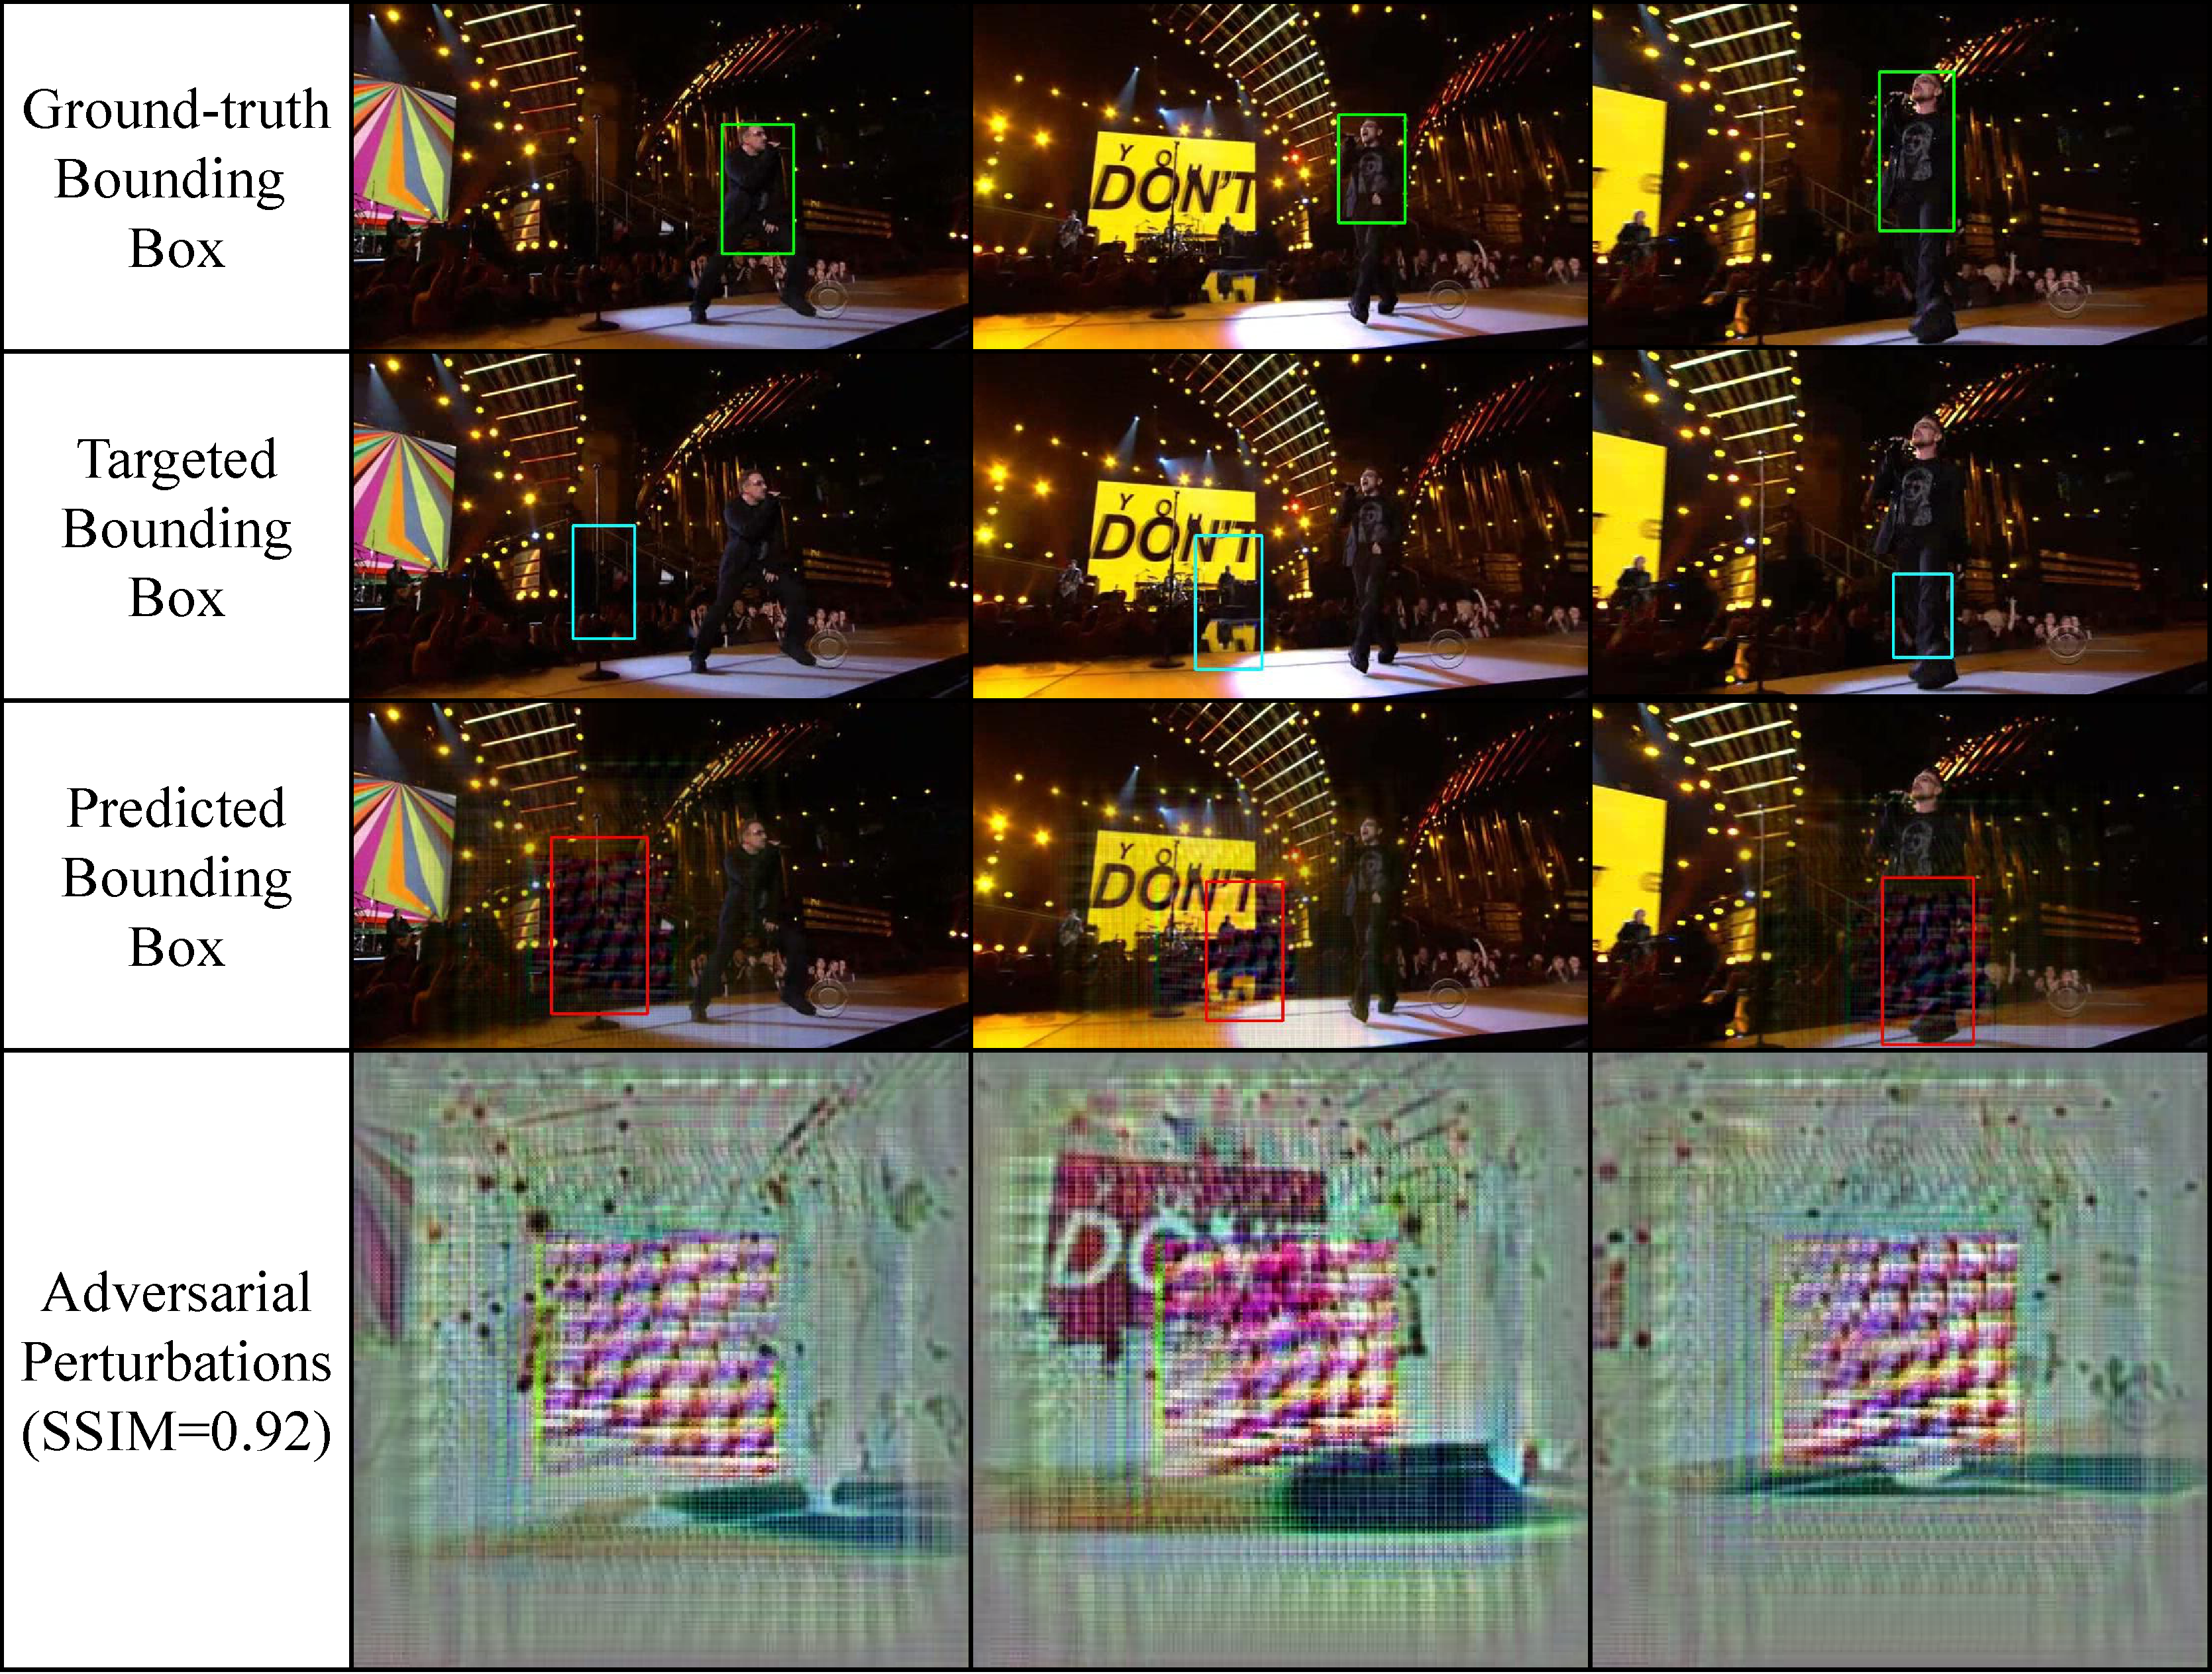
\includegraphics[width=0.48\textwidth]{FAN.pdf}}
    \subfigure[Ours]{\label{fig:b}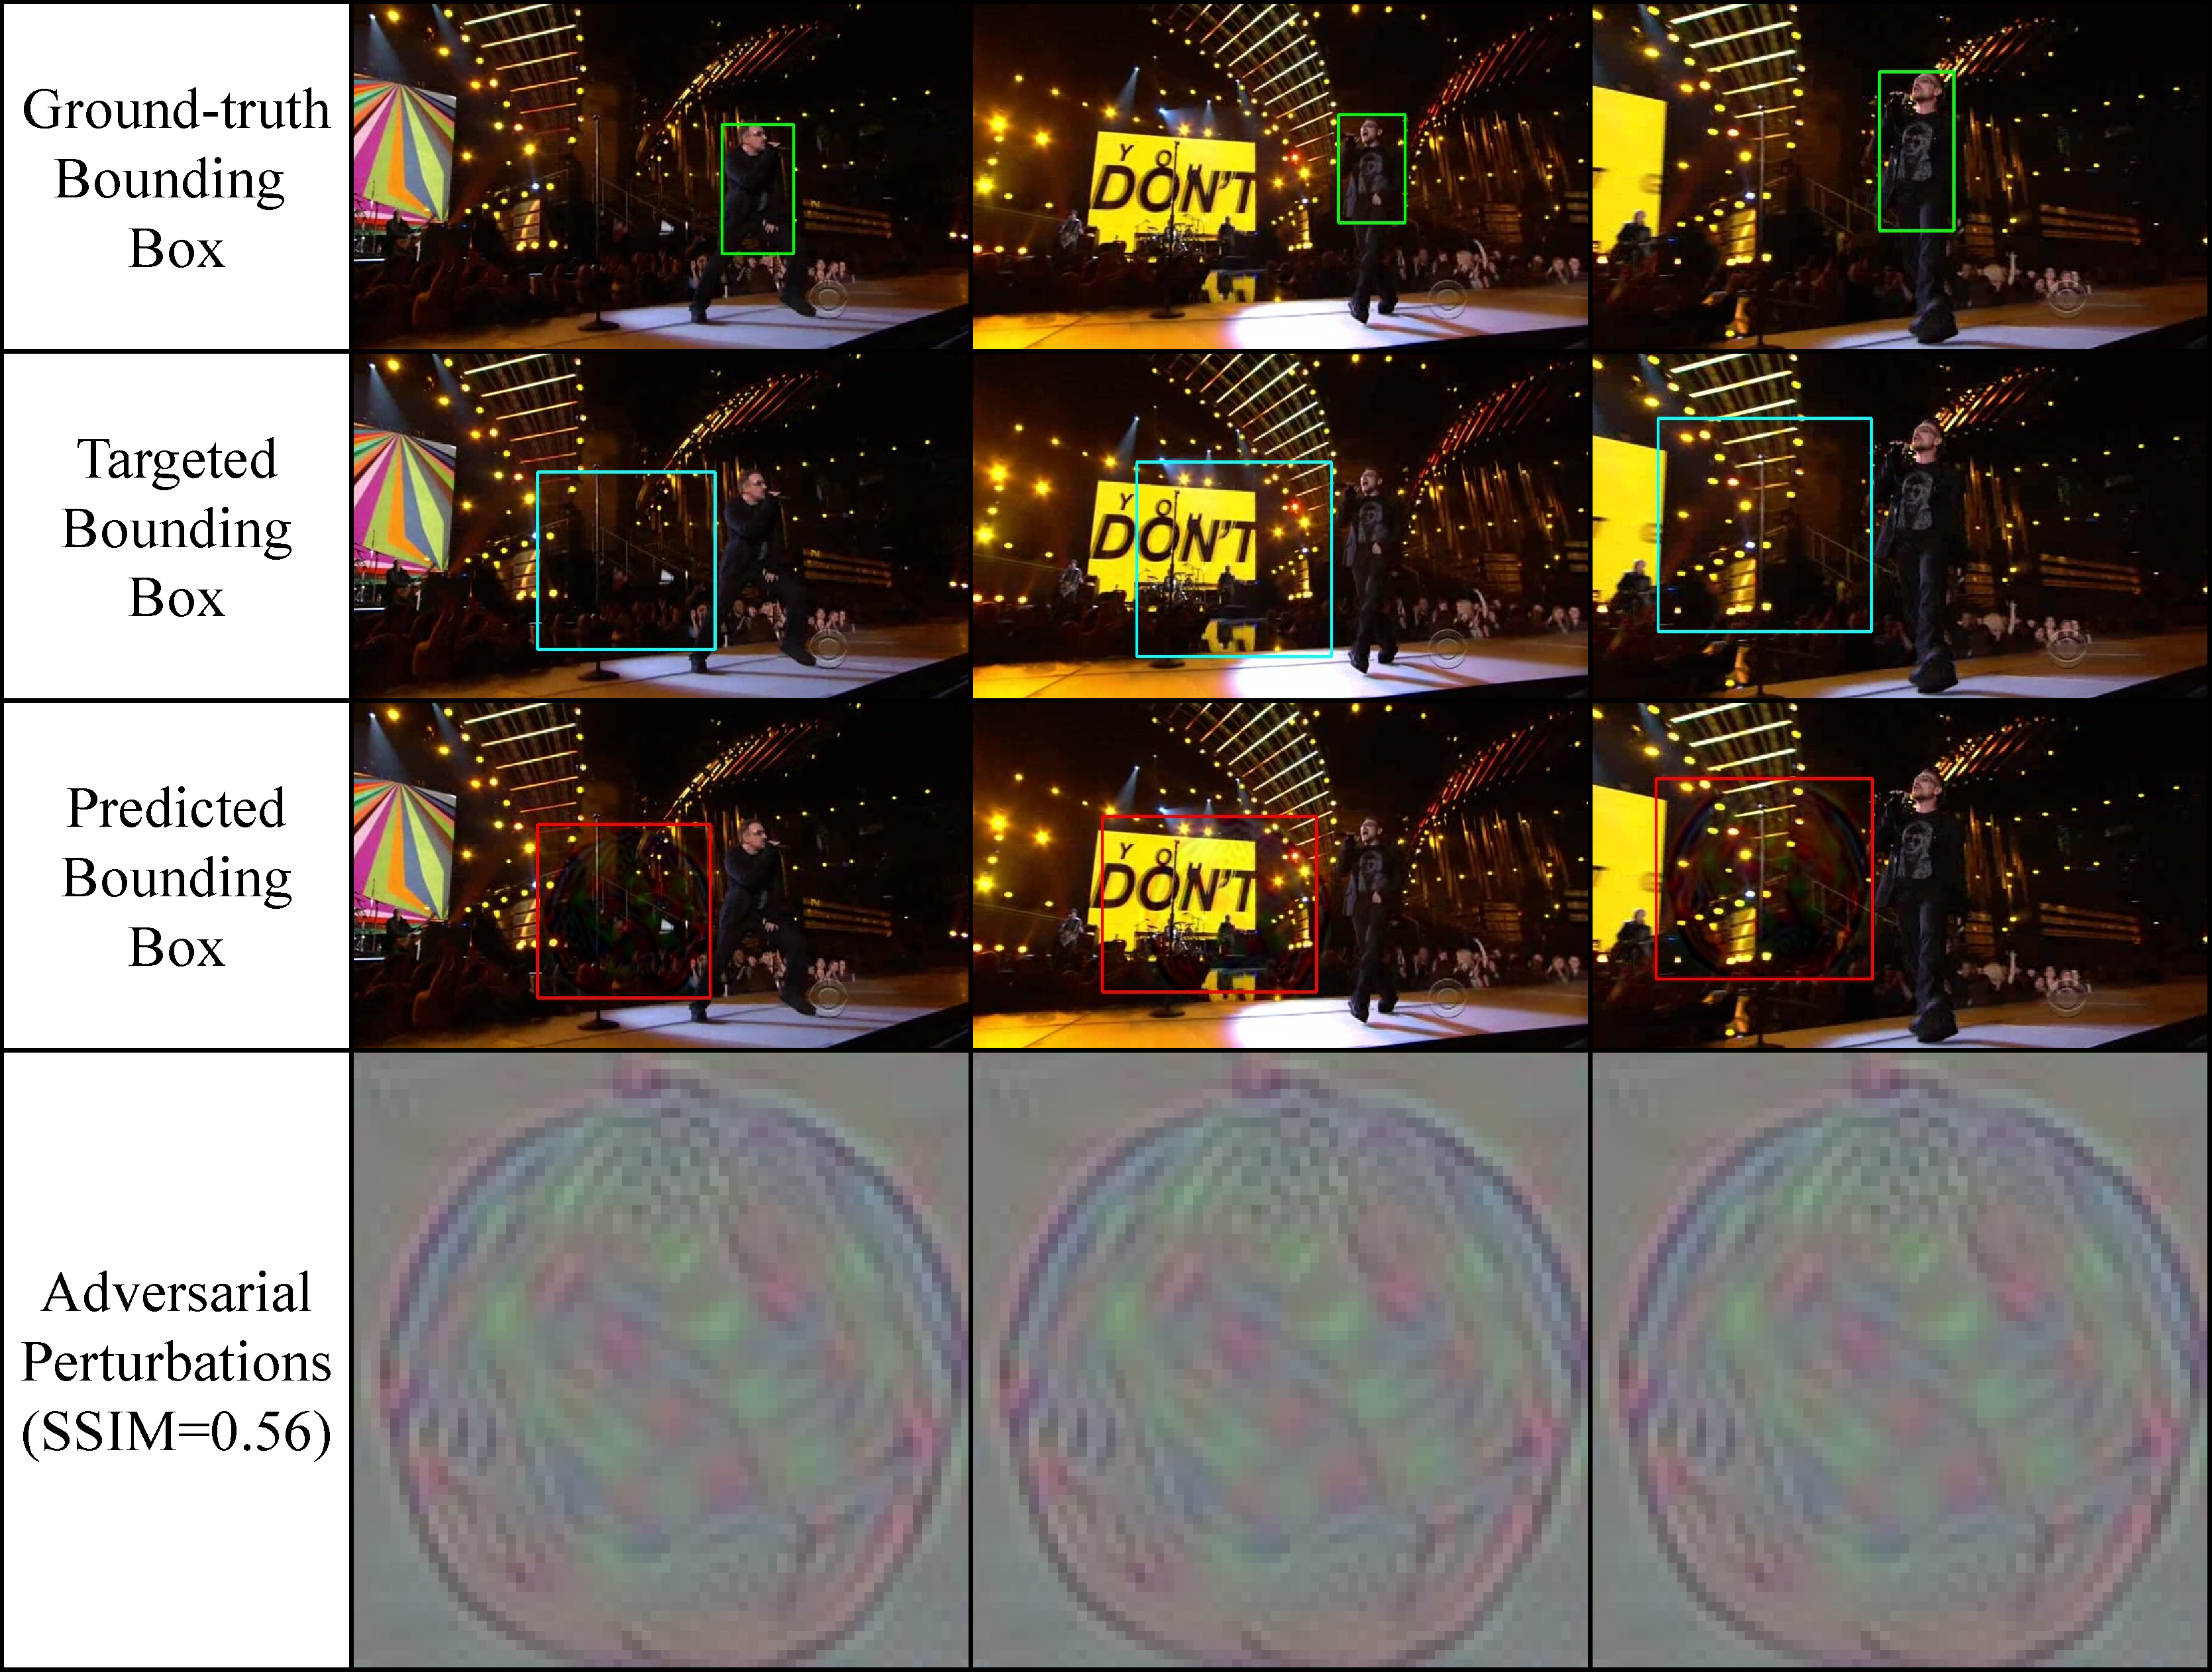
\includegraphics[width=0.48\textwidth]{Ours.pdf}}
    \caption{The results under targeted attacks compared with FAN \cite{FAN}.  FAN crafts the perturbations for each video independently, which comes at a non-negligible computational cost. To achieve video-agnostic universal attack on Siamese trackers, we relax the constraint on the value of the perturbation, achieving a balance between the attack efficiency and the perturbation perceptibility.}
    \label{fig:vis}
\end{figure}

\uline{
% 为了进一步分析扰动的可感知性,我们在图中与FAN进行了对比。
To further analyze the perceptibility of perturbations, we compare our method with FAN \cite{FAN} in Figure \ref{fig:vis}.
% We visualize the perturbed frames ($3^{rd}$ row of Figure \ref{fig:vis}) of OTB2015 dataset, Singer2 video. 
As shown in Figure \ref{fig:vis}, both FAN and our method can perform targeted attack. 
% 添加了由FAN生成的扰动的OTB的SSIM下降至0.92。添加了我们的扰动的OTB的SSIM下降至0.56。
The SSIM of OTB2015 perturbed by FAN drops to 0.92, while the SSIM perturbed by our method drops to 0.56.
% 这是因为FAN为每帧产生独立的扰动,而我们的扰动是通用的,因此我们的任务比FAN更难,导致我们的扰动值更大。
This is because FAN generates independent perturbations for each frame, while our perturbations are universal, which is a more difficult task, resulting in larger values for our perturbations.
By relaxing the constraint on the value of the perturbation, we can achieve better targeted attack performance on OTB2015.
Our method achieves a precision score of 0.795, compared to 0.420 for FAN.
What's more, our method can perform universal attack, both with respect to the data and the network architectures.}

% \begin{table*}[h]
%     \centering
%     \renewcommand\tabcolsep{5.5pt} % 调整表格列间的长度
%     \caption{Influence of the training iteration number on GOT-Val.}
%     \begin{tabular}{cc|ccccccccccccccc} 
%     \toprule
%     \multicolumn{2}{c|}{Iterations}     & 1     & 2     & 4     & 8     & 16    & 32    & 64    & 128   & 256   & 512   & 1024  & 2048  & 4096  & 8192  \\ 
%     \midrule
%     \multirow{2}{*}{Fake Traj.} & AO    &  0.14 & 0.14 & 0.14 & 0.14 & 0.14 & 0.14 & 0.15 & 0.18 & 0.47 & 0.73 & 0.78 & 0.82 & 0.84 & 0.84  \\
%                                 & SR    &  0.1 & 0.1 & 0.1 & 0.1 & 0.1 & 0.1 & 0.11 & 0.15 & 0.49 & 0.78 & 0.84 & 0.88 & 0.89 & 0.89    \\ 
%     \midrule
%     \multirow{2}{*}{Real Traj.} & AO   & 0.76 & 0.77 & 0.76 & 0.76 & 0.76 & 0.76 & 0.75 & 0.73 & 0.48 & 0.27 & 0.22 & 0.17 & 0.15 & 0.15    \\
%                                 & SR   & 0.89 & 0.9 & 0.89 & 0.89 & 0.9 & 0.89 & 0.88 & 0.86 & 0.53 & 0.25 & 0.18 & 0.14 & 0.12 & 0.12    \\ 
%     \midrule
%     \multicolumn{2}{c|}{SSIM of $\delta$}&   1 & 1 & 1 & 1 & 0.99 & 0.99 & 0.97 & 0.94 & 0.88 & 0.84 & 0.82 & 0.81 & 0.8 & 0.79\\
%     \midrule
%     % \multicolumn{2}{c|}{SSIM of $p$}      &  0.98 & 0.98 & 0.98 & 0.98 & 0.98 & 0.98 & 0.98 & 0.98 & 0.98 & 0.97 & 0.98 & 0.98 & 0.98 & 0.98\\
%     \multicolumn{2}{c|}{SSIM of $p$}      &  0.98 & 0.98 & 0.98 & 0.98 & 0.98 & 0.98 & 0.93 & 0.78 & 0.56 & 0.50 & 0.51 & 0.52 & 0.53 & 0.56\\
%     \bottomrule
%     \end{tabular}
%     \label{tab:iter}
% \end{table*}

%%%% 问题 2.2 %%%%
\textit{2. Your baseline approaches are not state-of-the-art algorithms. Why not compare to PAT \cite{PAT}, RTAA \cite{RTAA}, SPARK \cite{SPARK} and TTP \cite{TTP}. “However, RTAA only performs the untargeted attacks for trackers, which is less challenging than the targeted attacks in this paper, as we aim to create arbitrary, complex trajectories at test time.” If that is the case, it should be easy to achieve better performance than their approach. I think the experiments should including the methods of untargeted attack.}

\textbf{
Thanks for your advice and we have added experiments as you suggested. We have compared with state-of-the-art attack methods including RTAA, SPARK, TTP, CSA and FAN in both targeted and untargeted attack settings in Section IV. F. Specifically, we have removed the original Table VII included in Section IV.F of the previous manuscript, and added 2 new tables that demonstrate the untargeted and targeted attack results respectively. 
The table demonstrating the untargeted attack result is included in Section IV.F of the revised manuscript and referred to as Table \ref{tab:untargeted}.
The table demonstrating the targeted attack result is included in Section IV.F of the revised manuscript and referred to as Table \ref{tab:targeted}. 
% 我们没有与 PAT 对比,因为他们仅在私有数据上进行了实验,未在公开数据集上进行实验。
We do not compare with PAT because they only experimented on private data and not on the public datasets.
}

\begin{table}[h]
    \renewcommand\thetable{X} 
    \centering
    \caption{Untargeted attack: Precision score on OTB2015.}
    \begin{tabular}{@{}ccccc@{}}
    \toprule
    \multirow{2}{*}[-1pt]{Method} & \multirow{2}{*}[-1pt]{Tracker} & \multirow{2}{*}[-1pt]{\begin{tabular}[c]{@{}c@{}}Attack Cost\\per Frame(ms)\end{tabular}} & \multirow{2}{*}[-1pt]{\begin{tabular}[c]{@{}c@{}}Before\\ Attack\end{tabular}} & \multirow{2}{*}[-1pt]{Untargeted Attack} \\
        &  &  &  &     \\ \midrule
    RTAA & DaSiamRPN & - & 0.880 & 0.050\\
    SPARK & SiamRPN & 41.4 & 0.851 & 0.064\\
    CSA & SiamRPN & 9 & 0.851 & 0.458\\
    FAN & SiamFC & 10 & 0.720 & 0.180\\
    TTP & SiamRPN++ & 8 & 0.910 & 0.080 \\
    \midrule
    Ours & SiamFC++ & $\sim 0$ & 0.861 & 0.092\\ \bottomrule
    \end{tabular}
    \label{tab:untargeted}
\end{table}

\begin{table}[h]
    \renewcommand\thetable{XI} 
    \centering
    \caption{Targeted attack: Precision score on OTB2015.}
    \begin{tabular}{@{}ccc@{}}
    \toprule
    Method & Tracker &  Targeted Attack \\
    \midrule
    FAN & SiamFC  &0.420 \\
    TTP & SiamRPN++ &0.692 \\
    \midrule
    Ours & SiamFC++  &0.795 \\ \bottomrule
    \end{tabular}
    \label{tab:targeted}
\end{table}

\textbf{
As can be seen from Table \ref{tab:untargeted} and Table \ref{tab:targeted}, CSA reduces the accuracy score with respect to the real trajectory from 0.851 to 0.458. Due to the limitations of the algorithm design, CSA cannot perform targeted attacks for Siamese trackers. 
SPARK \cite{SPARK} reduces the accuracy score with respect to the real trajectory from 0.851 to 0.064. However, SPARK needs to generate distinct adversarial examples for every search image through heavy iterative schemes, which is time-consuming to attack online-tracking in real time.
RTAA \cite{RTAA} reduces the accuracy score with respect to the real trajectory from 0.880 to 0.050. However, RTAA only performs the untargeted attacks for trackers, which is less challenging than the targeted attacks in this paper, as we aim to create arbitrary, complex trajectories at test time. 
Recently, Liang et al. proposed a fast attack network (FAN) \cite{FAN} for attacking SiamFC trackers. To perform untargeted attacks, FAN proposes a drift loss that shifts the tracker's prediction of the target's position. The tracking error accumulates over time until the tracker loses the target completely. To perform targeted attacks, FAN proposes embedding feature loss for improving the similarity between the features of the adversarial sample and the features of regions specified by a particular trajectory. FAN can reduce the accuracy score with respect to the real trajectory from 0.720 to 0.180. However, the accuracy score with respect to fake trajectories is only 0.420. Similar to SCA, FAN also requires running a generative network for each frame to obtain adversarial information. 
Nakka et al. \cite{TTP} proposed the temporally transferable perturbations (TTP) for attacking the SiamRPN++ tracker. TTP generates a single adversarial perturbation from the template image and adds this perturbation to each search image of the video. TTP reduces the accuracy score with respect to the real trajectory from 0.910 to 0.080, which is effective for untargeted attacks. However, the accuracy score with respect to the fake trajectory is only 0.692, which demonstrates that TTP's performance of targeted attacks is limited. In addition, this method needs to run a generative network for each video to obtain adversarial information, thus requires the computational and storage resources of the object tracking platform, which makes it difficult to deploy the method to resource-constrained platforms. Our method can reduce the accuracy score with respect to real trajectories from 0.861 to 0.092. The accuracy score is up to 0.795 with respect to fake trajectories, which is significantly better than other methods, and only needs to perform the add operation to generate adversarial information for any video without gradient optimization or network inference.
}

\begin{table}[t]
    \renewcommand\thetable{IV} 
    \centering
    \caption{Overall attack results on VOT2016, VOT2018, VOT2019 and UAV123.}
    \begin{tabular}{c c | c | c}
    \toprule
    Benchmarks & Metrics & Before Attack    & Untargeted Attack  \\
    \midrule
    \multirow{2}{*}[-6pt]{VOT2016} 
    & Accuracy   & 0.626 & 0.393\\
    & Robustness & 0.144 & 9.061\\
    & EAO        & 0.460 & 0.007\\
    \midrule
    \multirow{2}{*}[-6pt]{VOT2018} 
    & Accuracy   & 0.587 & 0.342\\
    & Robustness & 0.183 & 8.981\\
    & EAO        & 0.426 & 0.007\\
    \midrule
    \multirow{2}{*}[-6pt]{VOT2019} 
    & Accuracy   & 0.556 & 0.345\\
    & Robustness & 0.537 & 8.824\\
    & EAO        & 0.243 & 0.010\\
    \midrule
    \multirow{3}{*}[+6pt]{UAV123} 
    & AO  & 0.623 & 0.064\\
    & Precision & 0.781 & 0.187\\
    \bottomrule
    \end{tabular}
    \label{tab:benchmark results1}
\end{table}

%%%% 问题 2.3 %%%%
\textit{3. “However, SPARK needs to generate distinct adversarial examples for every search image through heavy iterative schemes, which is time-consuming to attack online-tracking in real-time.” But you are not real-time as well. Why do you mention this part? You also didn’t show the response time of your system.}

\textbf{Sorry that in our previous manuscript we did not clarify that our perturbations are trained off-line and can perturb a novel video to come at no additional cost except the mere addition operations, not requiring gradient optimization or network inference, so we can attack online-tracking in real-time. The attack cost per frame is shown in Table \ref{tab:untargeted}.}

%%%% 问题 2.4 %%%%
\textit{4. There are some datasets adopted in \cite{SPARK,RTAA} that you should include in your experiments such as VOT2018, VOT2019, VOT2016, OTB2015 and UAV123. Otherwise, it is very difficult to justify the performance of the proposed method.}

\begin{table}[t]
    \renewcommand\thetable{V}
    \centering
    \caption{Overall attack results on OTB-15, GOT-Val and LaSOT.}
    \begin{tabular}{c c | c | c | c}
    \toprule
    \multirow{2}{*}[-2pt]{Benchmarks} & \multirow{2}{*}[-2pt]{Metrics} & Clean Videos    & \multicolumn{2}{c}{Perturbed Videos}  \\
    \cmidrule{3-5}
                              &                         & Real Traj. & Real Traj. & Fake Traj.     \\ 
    \midrule
    \multirow{2}{*}{OTB-15} 
    & AO   & 0.642 & 0.063 & 0.759\\
    & Precision & 0.861 & 0.092 & 0.795\\
    \midrule
    \multirow{2}{*}{GOT-Val} 
    & SR & 0.897 & 0.123 & 0.890\\
    & AO & 0.760 & 0.153 & 0.840 \\
    \midrule
    \multirow{3}{*}{LaSOT} 
    & Precision  & 0.514 & 0.046 & 0.605\\
    & Norm. Prec.& 0.551 & 0.048 & 0.702\\
    & AO         & 0.525 & 0.069 & 0.691\\
    %& Succ. rate  & 0.626 & 0.016 & 0.834\\
    \midrule
    \multicolumn{2}{c|}{FPS} & 58 & 58 & 58\\
    \bottomrule
    \end{tabular}
    \label{tab:benchmark results}
\end{table}

\textbf{Thanks for your advice and we have added experiments on VOT2018, VOT2016, OTB2015 and UAV123 in Section IV.D.
As suggested, we have added a new table that demonstrates the attack results on VOT2016, VOT2018, VOT2019 and UAV123. This new table is included in Section IV.D of the revised manuscript and referred to as Table IV. The table demonstrating the attack results on OTB2015, GOT-Val and LaSOT is included in Section IV.D of the revised manuscript and referred to as Table V.
% 新增加的实验结果分析位于某处,展示如下。
The detailed analysis of new added experiments is added in Section IV.D of the revised manuscript. For your convenience in cross-checking, the new text is given as follows.}

\uline{As shown in Table \ref{tab:benchmark results1}, the robustness on VOT2016, VOT2018 and VOT2019 increases rapidly after attacking the original sequences. The EAO drops dramatically from 0.460 to 0.007 on VOT2016 and from 0.426 to 0.007 on VOT2018. The AO drops from 0.623 to 0.064 on UAV123. The performance decrease indicates the effectiveness of our adversarial attack method.
In addition, the experimental results in Table \ref{tab:benchmark results1} show that our perturbations (trained from COCO, ILSVRC-VID and the training splits of GOT-10k and LaSOT) can perform effective attacks on different datasets including VOT2016, VOT2018, VOT2019 and UAV123. This demonstrates the transferability of the proposed method across different datasets.
}

%%%%%%%%%%%%%%%%% 审稿人 3 %%%%%%%%%%%%%%%%%
\clearpage
\newpage
{\centering\section*{Response Letter to Reviewer \#3}}
\noindent Dear Reviewer \#3:

Thank you very much for your thorough review. Your insightful comments are very helpful for us to improve the quality of the paper. According to your comments and suggestions, we have carefully and extensively revised the manuscript. The main revised parts are highlighted by underlines in the underlined version for your convenience. You will find that all your comments and suggestions are considered and followed. We hope that our revised manuscript is now appropriate for publication in IEEE Transactions on Circuits and Systems for Video Technology.
In addition, point-to-point responses to your comments are given below and highlighted using bold font in line with your comments in order to facilitate cross-referencing.\\[10pt]
\indent We are looking forward to your reply.\\[10pt]
\noindent Yours sincerely,\\
\noindent Zhenbang Li, Yaya Shi, Jin Gao, Shaoru Wang, Bing Li, Pengpeng Liang, Weiming Hu
\\
\\
\\
\noindent Dr. Jin Gao (Contact author)\\
\noindent National Laboratory of Pattern Recognition (NLPR)\\
\noindent Institute of Automation, Chinese Academy of Sciences (CASIA)\\
\noindent Address: No. 95, Zhongguancun East Road, Haidian District,\\
\noindent Beijing 100190, P. R. China\\
\noindent Email: jin.gao@nlpr.ia.ac.cn

\newpage
\textit{This paper aims to propose a universal targeted attack on Siamese visual tracking. The problem studied here is a classical adversarial attack problem where adversarial samples are generated to mislead the training process. The authors propose a simple approach to generate adversarial samples and use experiments to demonstrate the effectiveness of the proposed framework. The advantage of the proposed attack is computation efficient and can be used in the real-time video tracking.}

\textbf{Many thanks for your positive comments on the strength of our paper and the novelty of the proposed attack method.}

%%%% 问题 3.1 %%%%
\textit{However, I have the following questions listed below. 1. The authors use the concept of video agnostic, however, for the experiment, I do not see the experiments to demonstrate the video agnostic property of the proposed method. From my understanding, video agnostic property is that the adversarial examples generated from one dataset can be applied to another dataset. However, I do not see the experimental results to demonstrate this and the transferability across different datasets are required to demonstrate the performance of the proposed framework.}

\textbf{
We agree that the adversarial examples generated from one dataset should be applied to another dataset. So we add experiments to verify this. Specifically, we adopt COCO, ILSVRC-VID and the training splits of GOT-10k and LaSOT as our training set. The test set includes VOT2016, VOT2018, VOT2019 and UAV123.
Experimental results demonstrate the transferability of the proposed method across different datasets.
The detailed analysis of new added experiments is added in Section IV.D of the revised manuscript. For your convenience in cross-checking, the new text is given as follows.}

\uline{As shown in Table \ref{tab:benchmark results1}, the robustness on VOT2016, VOT2018 and VOT2019 increases rapidly after attacking the original sequences. The EAO drops dramatically from 0.460 to 0.007 on VOT2016 and from 0.426 to 0.007 on VOT2018. The AO drops from 0.623 to 0.064 on UAV123. The performance decrease indicates the effectiveness of our adversarial attack method.
In addition, the experimental results in Table \ref{tab:benchmark results1} show that our perturbations (trained from COCO, ILSVRC-VID and the training splits of GOT-10k and LaSOT) can perform effective attacks on different datasets including VOT2016, VOT2018, VOT2019 and UAV123. This demonstrates the transferability of the proposed method across different datasets.
}

%%%% 问题 3.2 %%%%
\textit{2. The paper attacks the video tracking assumed that the training data is available which in practice may not be available. Also, even though we know the video content only but without the ground truth box information, then how can we use the proposed approach to generate effective approach. If not, then the practicability of the approach is quite limited.}

% Our perturbations generate well on different datasets. Once trained on public datasets (i.e., COCO, ILSVRC-VID and the training splits of GOT-10k and LaSOT), the perturbations can effectively attack videos on VOT2016, VOT2018, VOT2019, UAV123, and OTB2015 (see Table \ref{tab:benchmark results1} and Table \ref{tab:benchmark results}). Thus, we can deploy perturbations trained on public datasets directly to real-world scenarios without fine-tuning using the private training set.

\textbf{
% 当数据集的标注信息不可用时,我们可以在视频上运行需要被攻击的跟踪器,为每帧预测一个跟踪框。预测的跟踪框可被视为 ground truth 用于训练我们的攻击算法。
When the ground truth box information of videos is not available, we can run the tracker (that needs to be attacked) on videos, generating one box for every frame. The predicted boxes can be considered as ground truth for training our attack method.
% 具体而言,我们使用 GOT-10k 训练集的视频,利用 SiamFC++ 预测跟踪结果。将得到的跟踪结果作为标签信息训练扰动,在 GOT-10k 验证集上进行评估。实验结果如表所示。
To verify this, we run SiamFC++ on videos in GOT-10k training set. The predicted bounding boxes are regarded as the ground truth box information of GOT-10k training set to train perturbations. We evaluate the attack performance on GOT-10k validation set.
The detailed analysis of new added experiments is added in Section IV.D of the revised manuscript. For your convenience in cross-checking, the new text is given as follows.}

\uline{\textit{Ablation Study: Performance w/o ground truth information} Our perterbations are trained using datasets with ground truth box information.
% 然而实际上我们可能仅知道视频内容而不知道边框信息。这时我们可以在视频上运行需要被攻击的跟踪器,为每帧预测一个跟踪框。预测的跟踪框可被视为 ground truth 用于训练我们的攻击算法。
However, we may only know the video content but without the ground truth box information in practice. When the ground truth box information of videos is not available, we can run the tracker (that needs to be attacked) on videos, generating one box for every frame. The predicted boxes can be considered as ground truth for training our attack method. To verify this, we run SiamFC++ on videos in GOT-10k training set. The predicted bounding boxes are regarded as the ground truth box information of GOT-10k training set to train perturbations. We evaluate the attack performance on GOT-10k validation set. Experimental results is shown in Table \ref{tab:agent}. 
% 使用GT训练结果是0.153, 不适用GT训练结果是0.160。
As can been seen in Table \ref{tab:agent}, the AO is 0.153 when the ground truth is used to train perturbations and 0.160 when the ground truth is not used.
% 因此,使用跟踪器预测结果代替 ground truth 进行训练是有效的。
Therefore, it is effective to use the predicted boxes instead of ground truth boxes for training perturbations.
}

\begin{table}
    \renewcommand\thetable{IX}
    \centering
    \caption{Attack results with or without ground truth (GT) information on GOT-Val.}
    \begin{tabular}{cccc}
        \toprule
        \multirow{2}{*}{Metrics} & \multirow{2}{*}{Before Attack} & \multicolumn{2}{c}{Untargeted Attack}                                            \\
                                 &                                & w/ GT information & w/o GT information \\ \midrule
        SR                       & 0.897                          & 0.123                                & 0.121                                     \\
        AO                       & 0.760                          & 0.153                                & 0.160                                     \\                              
        \bottomrule
    \end{tabular}
    \label{tab:agent}
\end{table}

\textit{3. The technical novelty of this paper is not high as it directly borrows the approach from the traditional adversarial attack and use two additional path to train the neural networks. Can the authors provide theoretical analysis to explain the effectiveness based on such small change?}

% 其他跟踪攻击方法是复杂的,需要设定专门的损失函数和优化方法。我们的攻击方法是简单的,不需要设定专门的损失函数和优化方法。其他攻击方法是非通用的,我们的跟踪方法是通用的。我们之所以能够以简单的方案实现更困难的通用攻击,主要是因为我们放松了对扰动值的限制。如图所示,FAN的SSIM为0.92,我们的扰动的SSIM为0.56。
\textbf{
(1) On one hand, other attack methods on Siamese trackers are complex and require specialized loss functions and optimization methods, while our method is simple and dose not require specialized loss functions and optimization methods.
On the other hand, other attack methods on Siamese trackers are not universal while our method are doubly universal, both with respect to the data and the network architectures.
The main reason why it is possible to implement more difficult universal attacks in a simple scheme is that we relax the constraint on the value of the perturbations, achieving a balance between the attack ability and the perturbation perceptibility.
As shown in Figure \ref{fig:vis}, both FAN \cite{FAN} and our method can perform targeted attack. 
% 添加了由FAN生成的扰动的OTB的SSIM下降至0.92。添加了我们的扰动的OTB的SSIM下降至0.56。
The SSIM of OTB2015 perturbed by FAN drops to 0.92, while the SSIM perturbed by our method drops to 0.56.
By relaxing the constraint on the value of the perturbation, we can achieve better targeted attack performance on OTB2015.
Our method achieves a precision score of 0.795, compared to 0.420 for FAN.
}

\textbf{
(2) To the best of our knowledge, our work is the first attempt to generate video-agnostic perturbations to attack Siamese trackers. Besides FGSM \cite{FGSM} and Brown et al.'s work \cite{patch}, other adversarial example generation methods such as C\&W \cite{carlini2017towards} and PGD \cite{PGD} can also be integrated into our attacking system to further improve the attack effect.
In short, we focus on proposing a video-agnostic attacking system for Siamese trackers instead of proposing a specific adversarial example generation method.}

\textbf{
(3) By studying the attack method of Siamese trackers, we argue that the disadvantage of Siamese trackers is that template matching-based tracking mechanism is vulnerable to attacks, i.e., if both the template and the search image are perturbed at the same time, then the tracking algorithm can easily be misled.
The implication for improving the tracking robustness is to make the tracker aware of the semantic information of the target being tracked, rather than relying on templates alone.}

\textit{4. I suggest the authors to add the table to summarize the characteristics of the used datasets.}

\textbf{Thanks for the insightful comment. As suggested, we have added a new table to summarize the characteristics of the used datasets.
The new table is included in Section IV.A of the revised manuscript and referred as Table \ref{tab:dataset}.}

\begin{table}[h]
    \renewcommand\thetable{I}
    \centering
    \renewcommand\tabcolsep{2.5pt} % 调整表格列间的长度
    \footnotesize
    \caption{Characteristics of the datasets used to train and evaluate the proposed attack method.}
    \begin{tabular}{lrccccc} \toprule
    \multicolumn{2}{c}{Dataset}                            & Videos & Total frames & Frame rate & Object classes & Num. of attributes \\ \midrule
    \multirow{4}{*}{Training set} & GOT-10k training split & 9.34K  & 1.4M        & 10 fps     & 480            & 6                  \\
                                  & LaSOT training split   & 1.12K  & 2.83M        & 30 fps     & 70             & 14                 \\
                                  & COCO2017               & n/a    & 118K         & n/a        & 80             & n/a                \\
                                  & ILSVRC-VID             & 5.4K   & 1.6M         & 30 fps     & 30             & n/a                \\ \midrule
    \multirow{7}{*}{Test set}     & GOT-10k validation split&180    & 21K          & 10 fps     & 84             & 6                  \\
                                  & UAV123                 & 123    & 113K         & 30 fps     & 9              & 12                 \\
                                  & LaSOT test split       & 280    & 690K         & 30 fps     & 70             & 14                 \\
                                  & OTB-15                 & 100    & 59K          & 30 fps     & 22             & 11                 \\
                                  & VOT2016                & 60     & 21K          & 30 fps     & 16             & 6                  \\
                                  & VOT2018                & 60     & 21K          & 30 fps     & 24             & 6                  \\ 
                                  & VOT2019                & 60     & 19K          & 30 fps     & 30             & 6                  \\ \bottomrule
    \end{tabular}
    \label{tab:dataset}
\end{table}

\textit{5. The paper contains some grammar mistakes and typos, the authors need to improve it by double check.}

\textbf{
Thanks for the good comment. We have carefully checked through the whole text and corrected the grammar mistakes and typos. 
Specifically, we have replaced ``Our perturbations also generalize well to SiamFC++-ShuffleNet, in despite of the customized components such as pointwise group convolution and channel shuffle operations in ShuffleNet.'' with}
``
\uline{Our perturbations also generalize well to SiamFC++-ShuffleNet, despite the customized components such as pointwise group convolution and channel shuffle operations in ShuffleNet.}
''
\textbf{in Section IV.E of the revised manuscript.}

\textbf{
We have replaced ``SPARK computes incremental perturbations by using information from the past frames to perform targeted attacks to Siamese trackers.'' with}
``
\uline{SPARK computes incremental perturbations by using information from the past frames to perform targeted attacks on Siamese trackers.}
''
\textbf{in Section II.B of the revised manuscript.}

\normalem
\bibliographystyle{IEEEtran}
\bibliography{ref.bib}

\end{document}

